\documentclass[border=10pt]{standalone}
\usepackage{tikz}
\usepackage{booktabs}
\usepackage{array}
\usetikzlibrary{arrows.meta, positioning}
\definecolor{nodecolor}{RGB}{59, 130, 246}
\definecolor{fingercolor}{RGB}{168, 85, 247}

\begin{document}
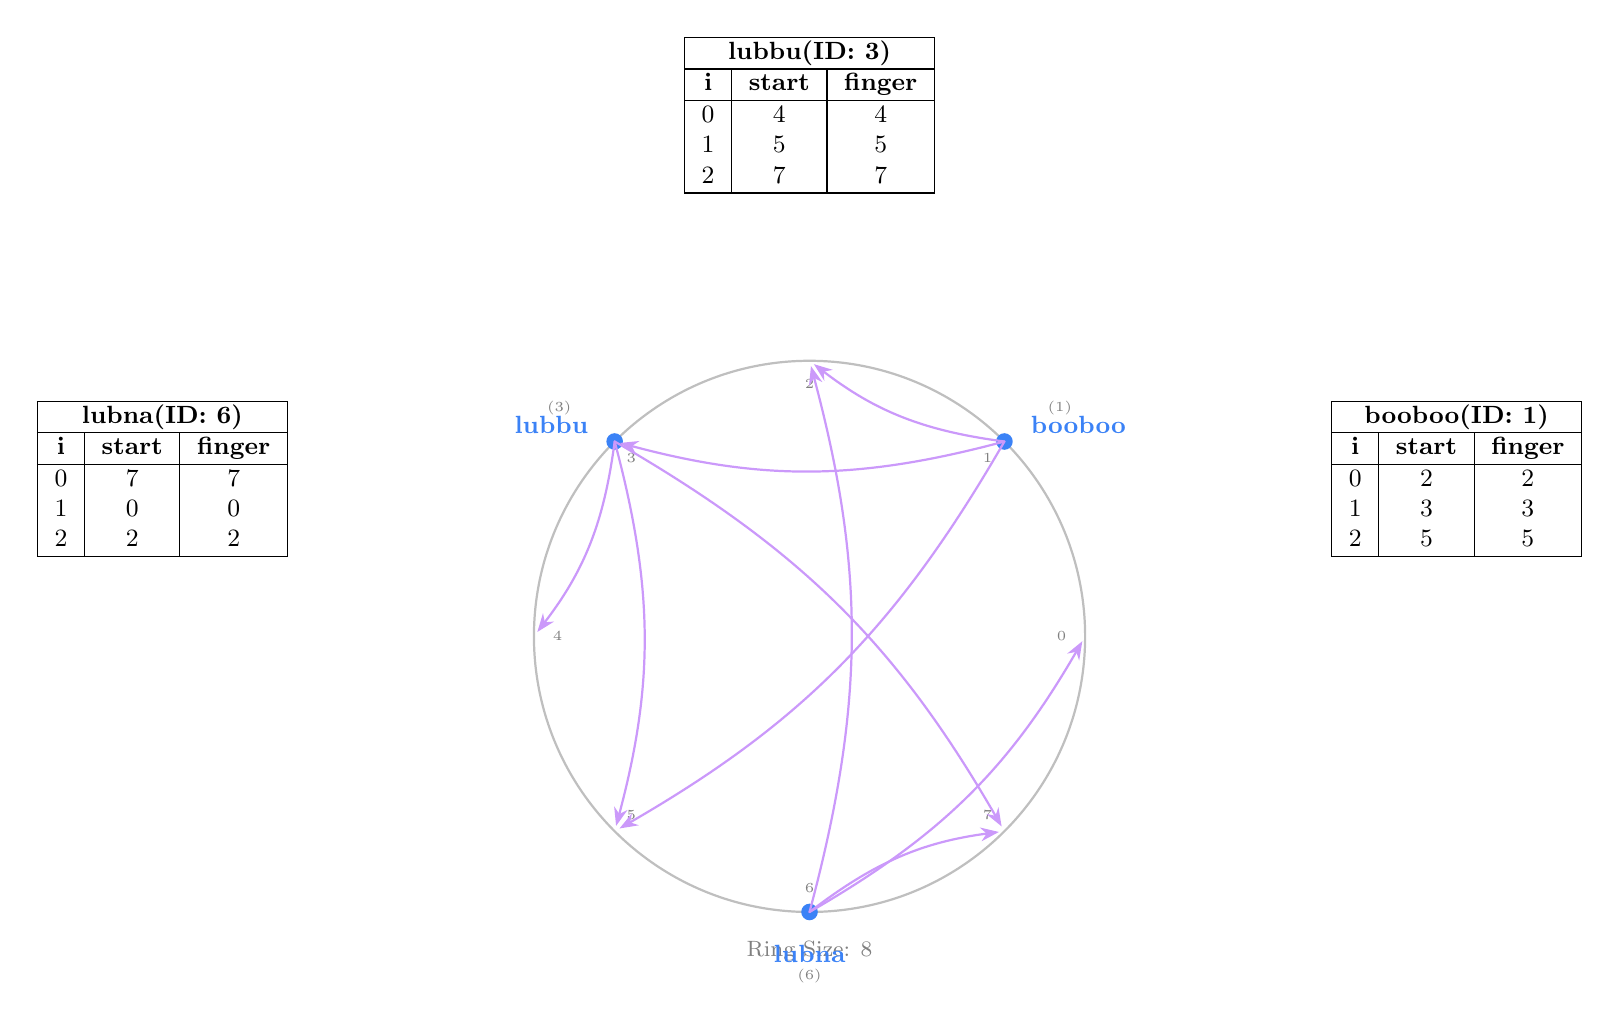
\begin{tikzpicture}[>=Stealth, line cap=round, line join=round]
  
  % Draw the ring
  \def\R{3.5}
  \draw[thick, gray!50] (0,0) circle (\R);
  
  % Ring size annotation
  \node[gray, font=\footnotesize] at (0, -\R-0.5) {Ring Size: 8};
  
  % Label circle with IDs
  \node[gray, font=\tiny] at (0:3.2) {0};
  \node[gray, font=\tiny] at (45:3.2) {1};
  \node[gray, font=\tiny] at (90:3.2) {2};
  \node[gray, font=\tiny] at (135:3.2) {3};
  \node[gray, font=\tiny] at (180:3.2) {4};
  \node[gray, font=\tiny] at (225:3.2) {5};
  \node[gray, font=\tiny] at (270:3.2) {6};
  \node[gray, font=\tiny] at (315:3.2) {7};
  
  
  % Draw nodes on the circle
  \fill[nodecolor] (270:3.5) circle (3pt);
  \node[nodecolor, font=\bfseries\small, anchor=north] at (270:3.8) {lubna};
  \node[gray, font=\tiny, anchor=north] at (270:4.1) {(6)};
  \fill[nodecolor] (135:3.5) circle (3pt);
  \node[nodecolor, font=\bfseries\small, anchor=east] at (135:3.8) {lubbu};
  \node[gray, font=\tiny, anchor=east] at (135:4.1) {(3)};
  \fill[nodecolor] (45:3.5) circle (3pt);
  \node[nodecolor, font=\bfseries\small, anchor=west] at (45:3.8) {booboo};
  \node[gray, font=\tiny, anchor=west] at (45:4.1) {(1)};
  
  
  % Draw finger table arrows
  \draw[->, fingercolor!60, thick, shorten >=2pt] (270.0:3.5) 
    to[bend left=15] (315.0:3.5);
  \draw[->, fingercolor!60, thick, shorten >=2pt] (270.0:3.5) 
    to[bend right=15] (0.0:3.5);
  \draw[->, fingercolor!60, thick, shorten >=2pt] (270.0:3.5) 
    to[bend right=15] (90.0:3.5);
  \draw[->, fingercolor!60, thick, shorten >=2pt] (135.0:3.5) 
    to[bend left=15] (180.0:3.5);
  \draw[->, fingercolor!60, thick, shorten >=2pt] (135.0:3.5) 
    to[bend left=15] (225.0:3.5);
  \draw[->, fingercolor!60, thick, shorten >=2pt] (135.0:3.5) 
    to[bend left=15] (315.0:3.5);
  \draw[->, fingercolor!60, thick, shorten >=2pt] (45.0:3.5) 
    to[bend left=15] (90.0:3.5);
  \draw[->, fingercolor!60, thick, shorten >=2pt] (45.0:3.5) 
    to[bend left=15] (135.0:3.5);
  \draw[->, fingercolor!60, thick, shorten >=2pt] (45.0:3.5) 
    to[bend left=15] (225.0:3.5);
  
  
  % Finger tables positioned around the circle
  \node[anchor=east, font=\small] at (-6.5, 2) {
    \begin{tabular}{|c|c|c|}
    \hline
    \multicolumn{3}{|c|}{\textbf{lubna(ID: 6)}} \\
    \hline
    \textbf{i} & \textbf{start} & \textbf{finger} \\
    \hline
    0 & 7 & 7 \\
    1 & 0 & 0 \\
    2 & 2 & 2 \\
    \hline
    \end{tabular}
  };
  \node[anchor=south, font=\small] at (0, 5.5) {
    \begin{tabular}{|c|c|c|}
    \hline
    \multicolumn{3}{|c|}{\textbf{lubbu(ID: 3)}} \\
    \hline
    \textbf{i} & \textbf{start} & \textbf{finger} \\
    \hline
    0 & 4 & 4 \\
    1 & 5 & 5 \\
    2 & 7 & 7 \\
    \hline
    \end{tabular}
  };
  \node[anchor=west, font=\small] at (6.5, 2) {
    \begin{tabular}{|c|c|c|}
    \hline
    \multicolumn{3}{|c|}{\textbf{booboo(ID: 1)}} \\
    \hline
    \textbf{i} & \textbf{start} & \textbf{finger} \\
    \hline
    0 & 2 & 2 \\
    1 & 3 & 3 \\
    2 & 5 & 5 \\
    \hline
    \end{tabular}
  };
  
  
\end{tikzpicture}
\end{document}
